\appendix{Представление графического материала}

Графический материал, выполненный на отдельных листах,
изображен на рисунках А.1--А.\arabic{числоПлакатов}.
\setcounter{числоПлакатов}{0}

\renewcommand{\thefigure}{А.\arabic{figure}} % шаблон номера для плакатов

\begin{landscape}

\begin{плакат}
    
\includegraphics[width=0.82\linewidth]{plakat1.eps}
    \заголовок{Сведения о ВКРБ}
    \label{pl1:image}      
\end{плакат}

\begin{плакат}
    
\includegraphics[width=0.82\linewidth]{plakat2.eps}
    \заголовок{Цель и задачи разработки}
    \label{pl2:image}      
\end{плакат}

\begin{плакат}
    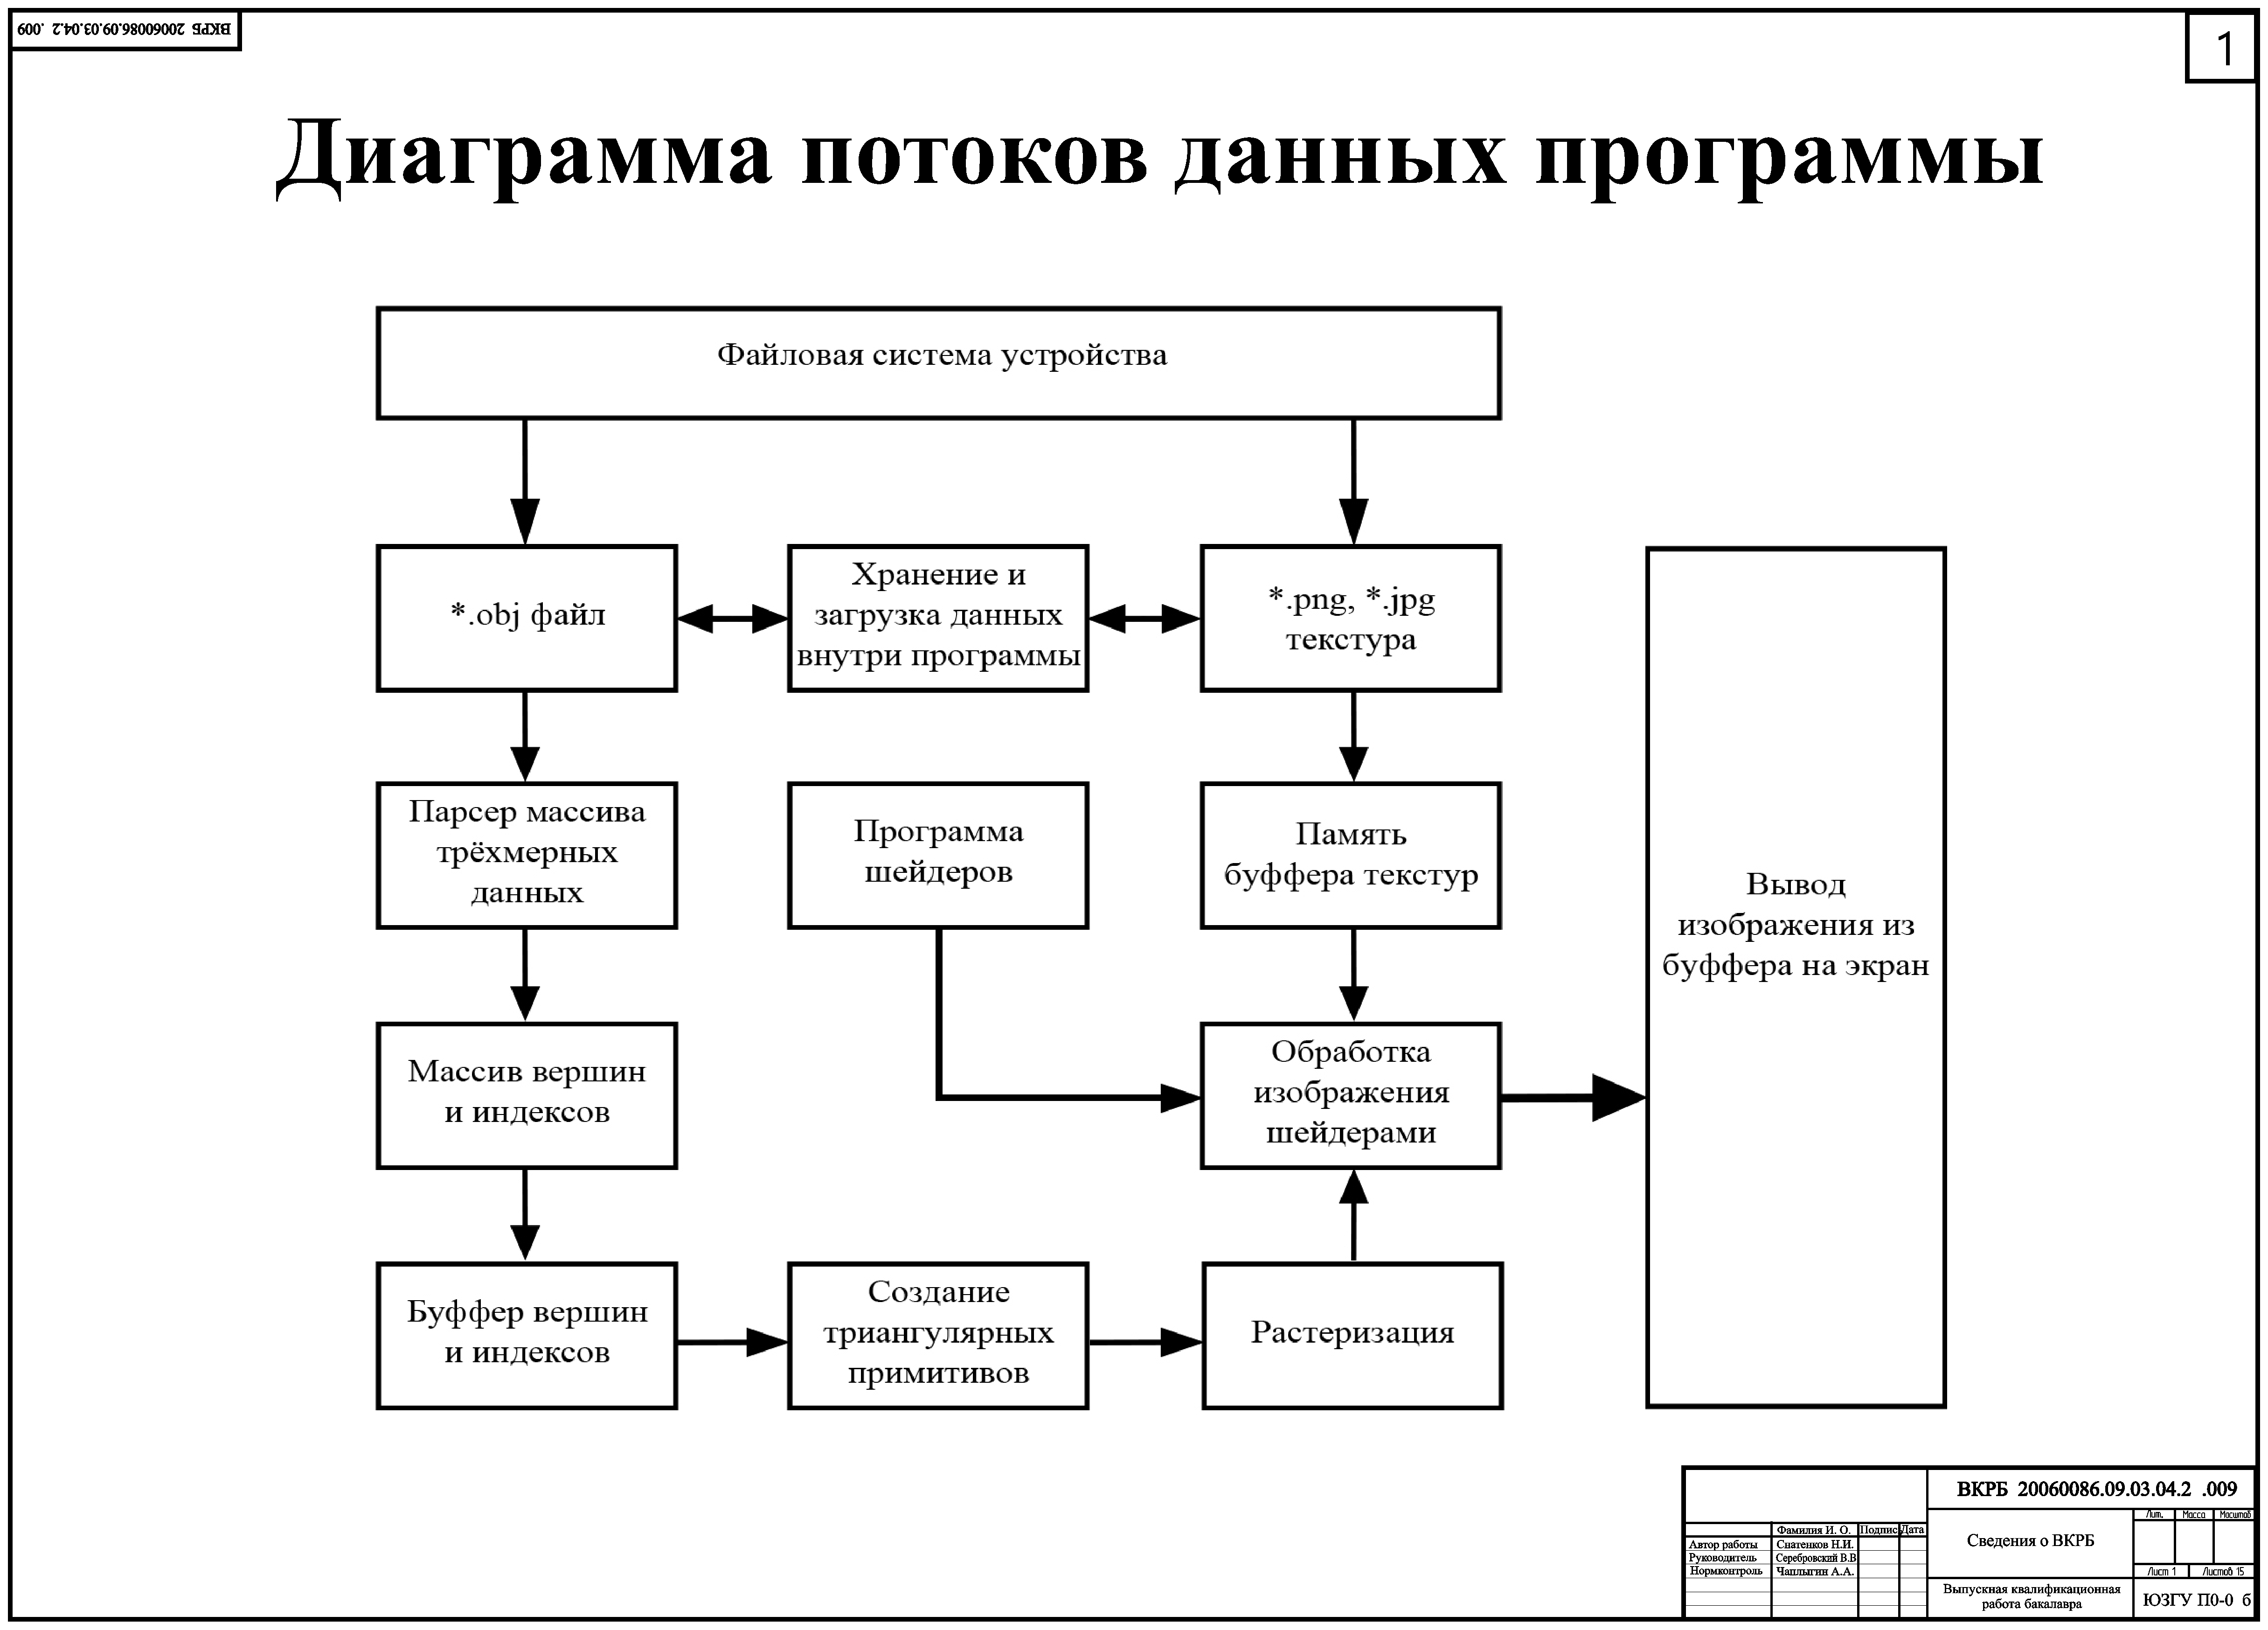
\includegraphics[width=0.82\linewidth]{plakat3.eps}
    \заголовок{Диаграмма конвеера данных}
    \label{pl3:image}      
\end{плакат}

\begin{плакат}
    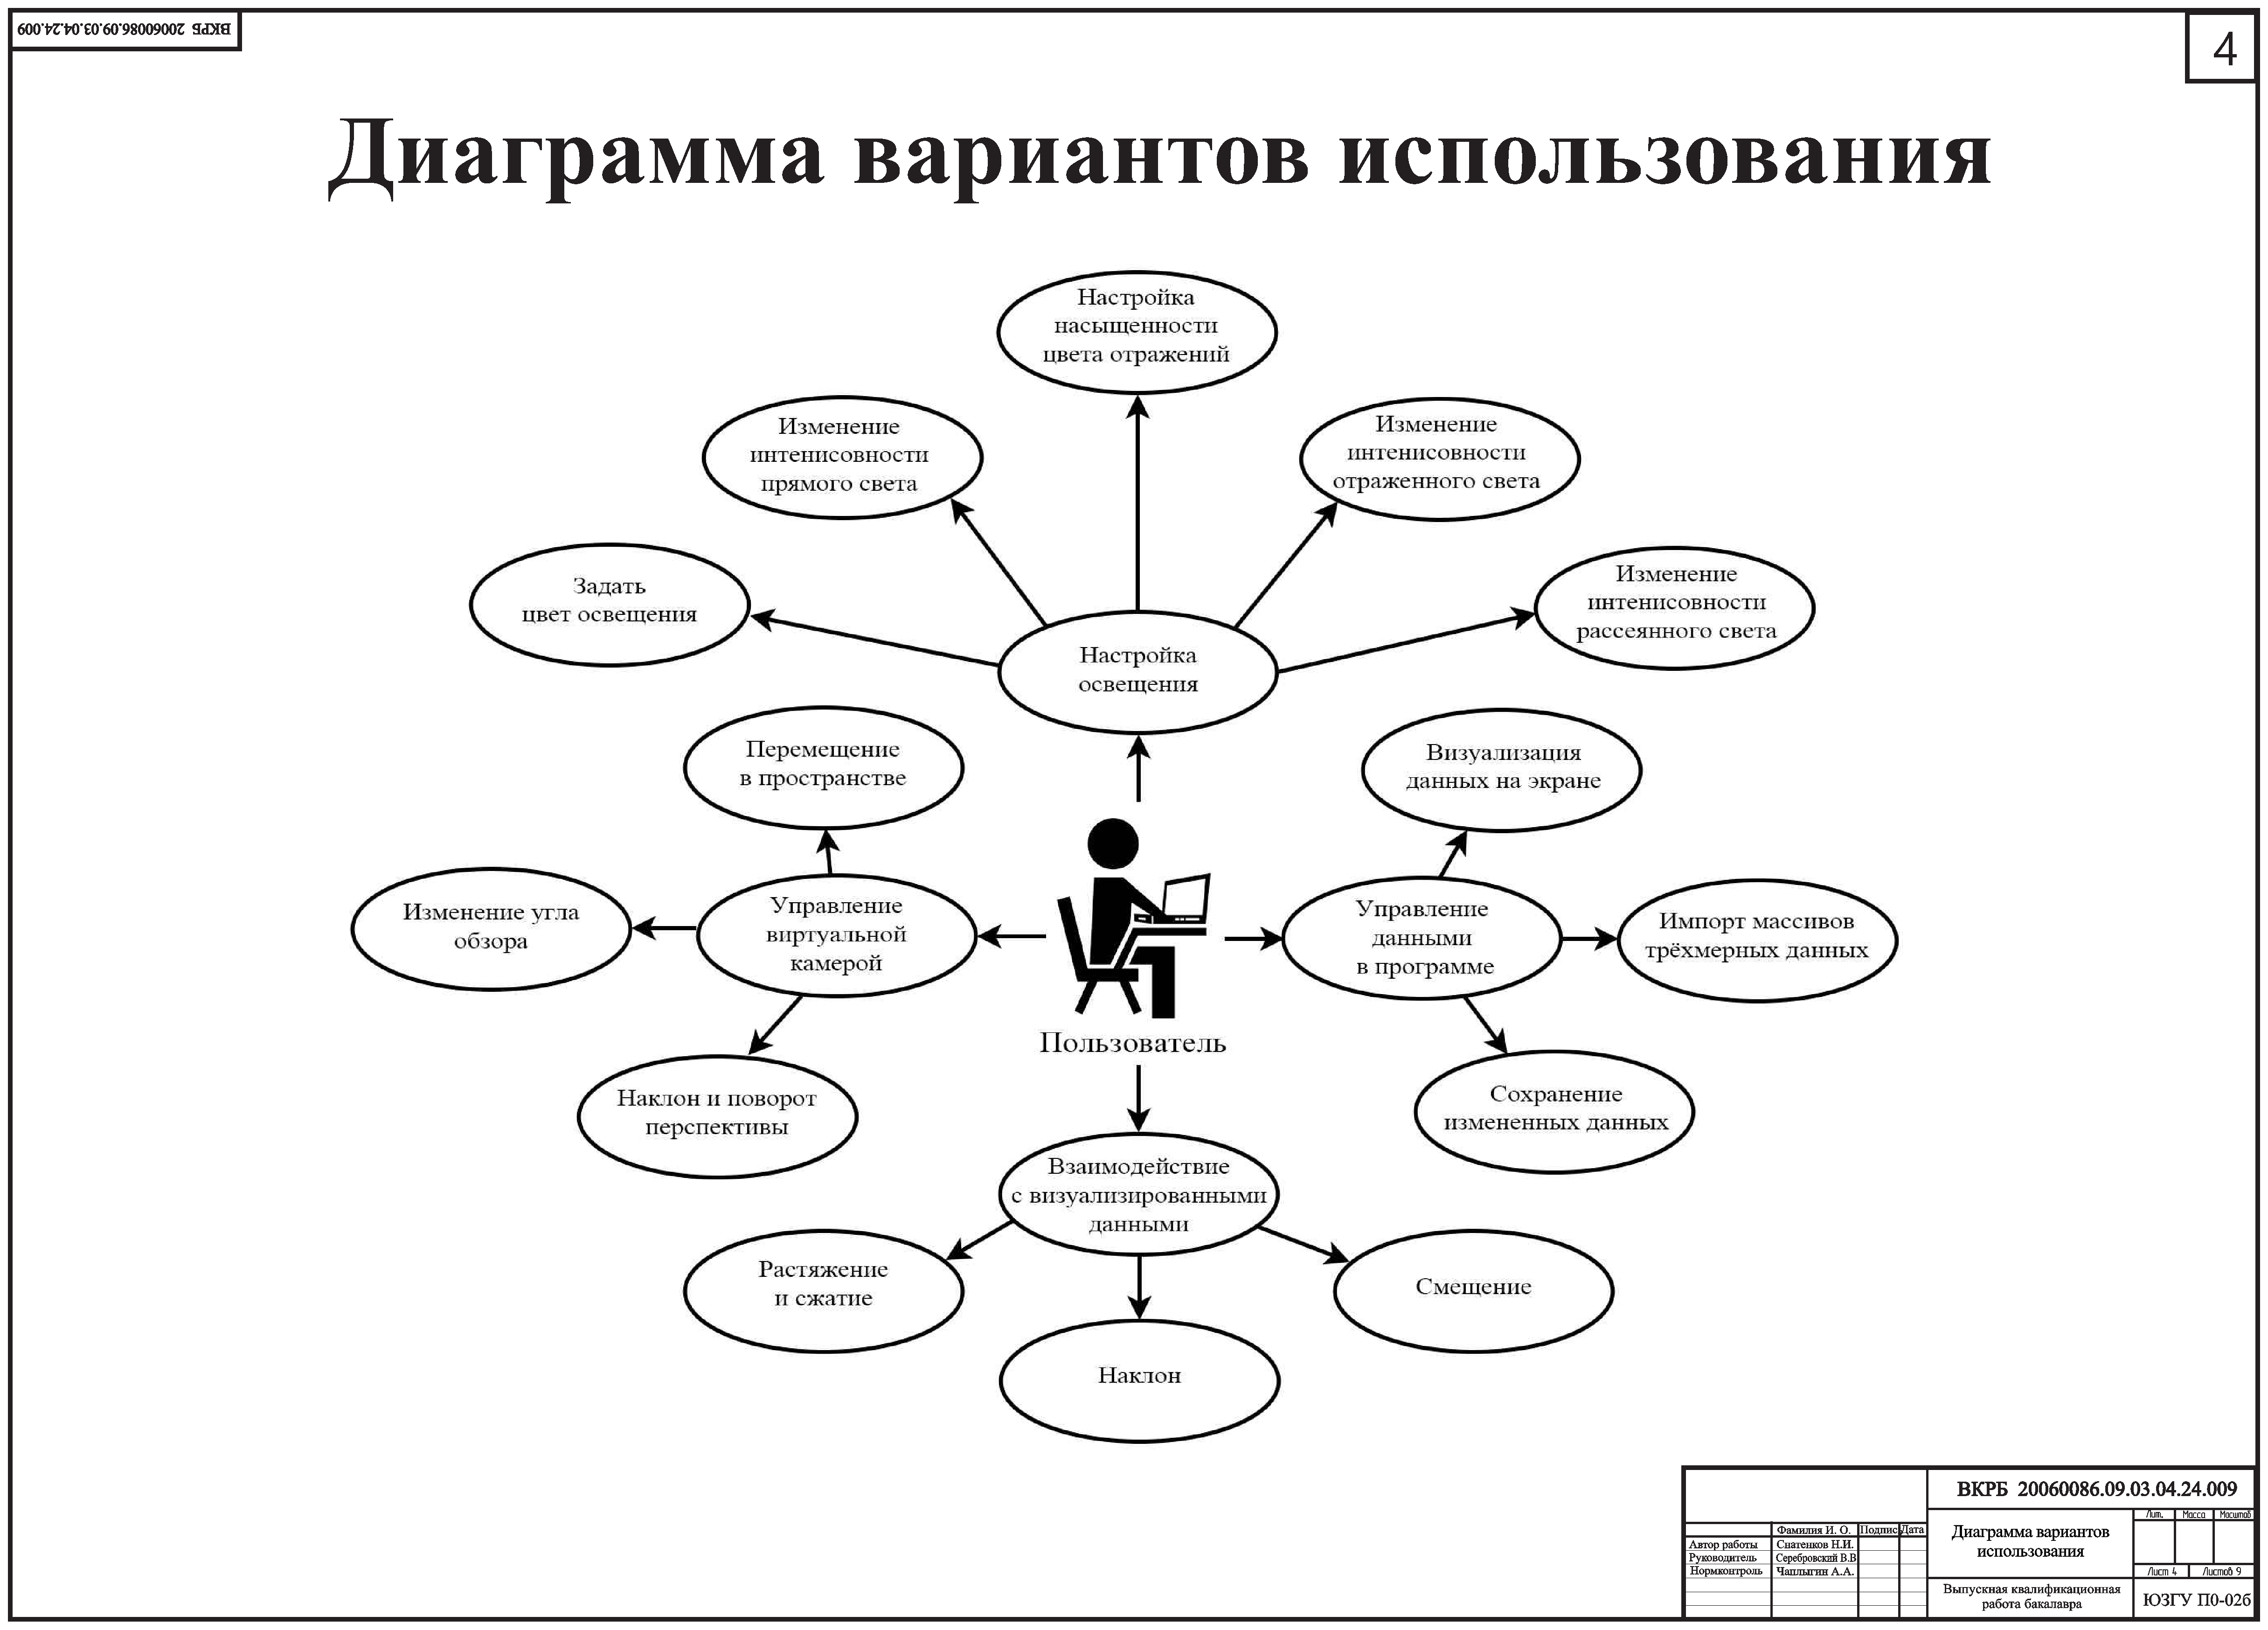
\includegraphics[width=0.82\linewidth]{plakat4.eps}
    \заголовок{Диаграмма вариантов использования}
    \label{pl4:image}      
\end{плакат}

\begin{плакат}
	
\includegraphics[width=0.82\linewidth]{plakat5.eps}
	\заголовок{Диаграмма классов программы}
	\label{pl5:image}      
\end{плакат}

\begin{плакат}
	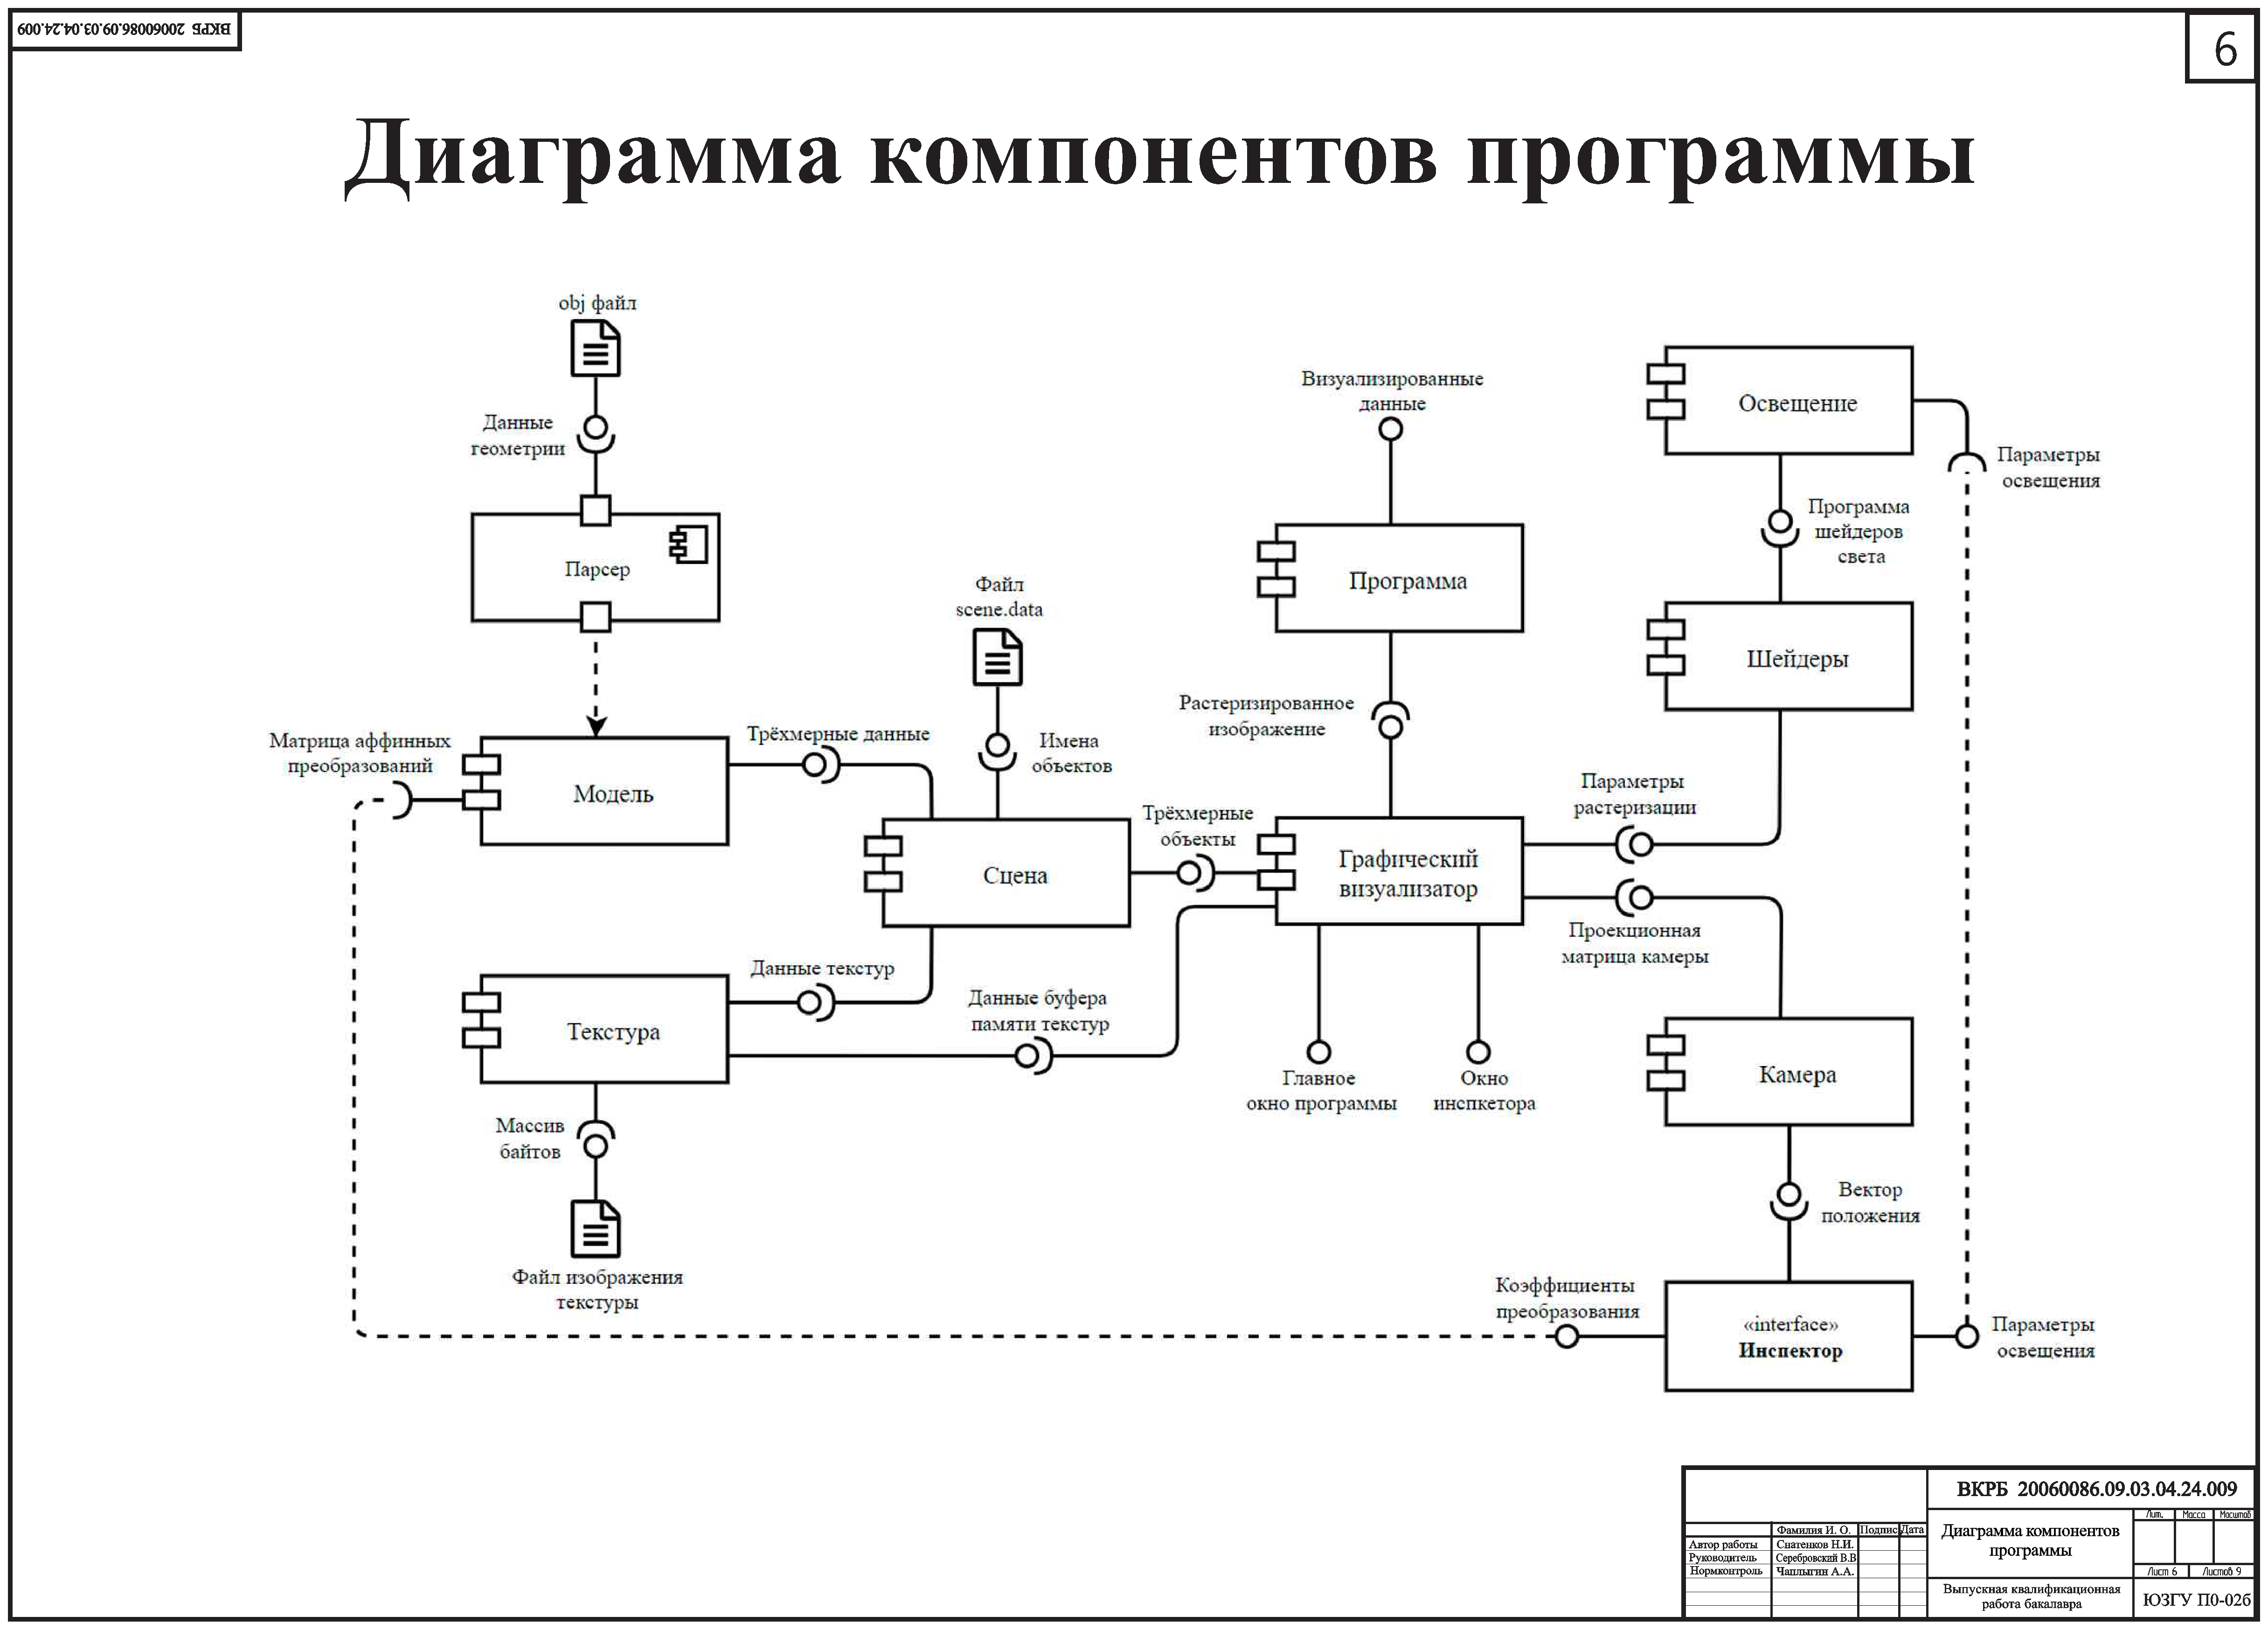
\includegraphics[width=0.82\linewidth]{plakat6.eps}
	\заголовок{Прототип компонентов программы}
	\label{pl6:image}      
\end{плакат}

\begin{плакат}
	
\includegraphics[width=0.82\linewidth]{plakat7.eps}
	\заголовок{Прототип интерфейса программы}
	\label{pl7:image}      
\end{плакат}

\begin{плакат}
	
\includegraphics[width=0.82\linewidth]{plakat8.eps}
	\заголовок{Интерфейс программы}
	\label{pl8:image}      
\end{плакат}

\begin{плакат}
	
\includegraphics[width=0.82\linewidth]{plakat9.eps}
	\заголовок{Результат визуализации трёхмерных данных}
	\label{pl9:image}      
\end{плакат}

\end{landscape}
